\documentclass{tietreport}

% Import images
\usepackage{graphicx}

% Packages required by the report tables and UML figure placement.
% The supplied TIET class controls all document formatting.
\usepackage{booktabs}
\usepackage{tabularx}
\usepackage{float}
\usepackage{pdflscape}

\usepackage[
  date=year,
  style=alphabetic,
  backend=biber,
  sorting=nty,
  maxnames=5,
  minnames=3,
  maxalphanames=4,
  minalphanames=3,
  backref=true,
  doi=false,
  isbn=false,
  url=true,
  eprint=false
]{biblatex}
\usepackage{xurl}
\hypersetup{hidelinks}
\addbibresource{references.bib}
\AtBeginBibliography{\raggedright}

\graphicspath{{../docs/diagrams/rendered/}}

\TitlePageHeader{UCS503 - Software Engineering}
\ProjectTitle{BharatOS}
\ProjectSubTitle{A Unified Civic Data Discovery and Developer API Platform}
\author{%
  \texttt{1024240135} Shivansh Singh \\
  \texttt{1024240155} Palveen Kaur \\
  \texttt{1024240106} Rajuss Sachdev \\
  \texttt{1024240006} Shivam Chauhan%
}
\TitlePageSubText{%
  Group: \texttt{To be confirmed} \\
  B.E. Third Year, Computer Science and Engineering \\
  Academic Year 2026--27, Odd Semester%
}
\AdvisorName{To be confirmed}
\TitlePageFooterText{{%
  \large Software Engineering Lab Report \\[0.2cm]
  \bfseries Computer Science and Engineering Department%
} \\[0.15cm]
Thapar Institute of Engineering and Technology, Patiala}

\begin{document}

\maketitle

\chapter*{Abstract}
\addcontentsline{toc}{chapter}{Abstract}
BharatOS is a Python-first academic prototype that reduces the effort required to discover
Indian public schemes and integrate permitted civic data. Government information is
distributed across portals with different formats, field names, update schedules and access
patterns. The proposed platform places a common discovery and normalization layer above
those official sources while preserving source attribution and freshness metadata.

Phase 1 implements a responsive citizen portal, scheme-detail pages, a developer console,
API documentation, a clearly labelled administrator preview and three versioned REST
endpoints. The implementation uses FastAPI, Jinja, Pydantic, custom CSS and minimal
JavaScript. Eight scheme snapshots and three PIN-code records are maintained in memory and
are explicitly labelled as prototype data. A visible demonstration key protects the API only
to prove the request contract; production authentication, PostgreSQL, Redis and scheduled
ingestion are intentionally deferred. Nineteen automated tests pass, and desktop/mobile
browser checks confirm the primary flows. Five UML diagrams document requirements,
structure, behaviour, processing and deployment-level components of the target system.

\textbf{Keywords:} civic technology, government schemes, FastAPI, REST API, data
normalization, provenance, UML, software engineering.

\tableofcontents
\listoffigures
\listoftables

\chapter{Introduction}

\section{Background and Context}
India publishes substantial civic and administrative information through ministry portals,
the Open Government Data platform, API Setu and other official systems. Availability alone,
however, does not guarantee developer accessibility. Sources often use different formats,
field names, authentication methods and update schedules. Citizens face a similar discovery
problem when they must visit many websites to identify potentially relevant schemes.

BharatOS addresses this fragmentation through two complementary interfaces. Citizens receive
anonymous search and filtering over source-linked scheme summaries. Developers receive a
versioned REST contract with predictable success and error envelopes. Official publishers
remain authoritative; BharatOS is an academic discovery and normalization layer rather than
a replacement for government portals. The myScheme platform, the Open Government Data
PIN-code directory and PFRDA pages are used only as source references for the small prototype
snapshot~\cite{myscheme,ogdpincode,pfrdaapy}.

\subsection{Problem Statement}
Developers and citizens can spend more time locating, interpreting and reconciling government
information than using it. Equivalent concepts may have different names, schemas, file formats
and freshness indicators. There is no single course-scale interface that demonstrates how
these records can be normalized, attributed and exposed safely.

\textbf{Problem:} How can permitted Indian public schemes and civic data be presented through
a single, source-transparent discovery portal and a consistent developer API without implying
official status or collecting unnecessary personal information?

\section{Project Objectives}
\begin{enumerate}
  \item Build a responsive localhost interface containing public discovery, scheme details,
        developer tooling, API documentation and an administrator preview.
  \item Define typed canonical models and versioned API envelopes using Python and Pydantic.
  \item Provide three executable prototype endpoints with consistent key validation and errors.
  \item Attach official source links, verification dates and freshness labels to every record.
  \item Model the complete target system with semantically correct and editable UML diagrams.
  \item Verify the implementation through automated tests and browser-level desktop/mobile review.
  \item Plan database, ingestion, authentication, caching, monitoring and deployment work in
        independently verifiable phases.
\end{enumerate}

\section{Scope and Phase Boundary}
Phase 1 validates the user experience, data contract and architecture. It includes eight
manually curated scheme records, three PIN-code records and a fixed public demonstration key.
It does not claim live ingestion, final eligibility decisions, persistent accounts, rate
limiting, PostgreSQL, Redis, production security or measured load-test performance. This
boundary prevents prototype behaviour from being confused with completed production features.

\chapter{Requirements Analysis}

\section{Stakeholders and Actors}
\begin{table}[H]
\centering
\begin{tabularx}{\textwidth}{@{}lXX@{}}
\toprule
\textbf{Actor} & \textbf{Role} & \textbf{Primary interactions} \\
\midrule
Public User & Uses public features without creating an account. & Search and filter schemes,
view details, inspect provenance, review potential fit and look up PIN codes. \\
Registered Developer & Specializes the public user with developer credentials. & Sign in,
manage keys, call APIs, test endpoints and view usage. \\
Administrator & Operates the platform. & Manage sources, trigger ingestion, monitor freshness
and review abuse. \\
Government Data Source & External publisher of permitted records. & Supplies API responses or
documented snapshots to ingestion. \\
Scheduler & External time-based trigger. & Starts scheduled ingestion runs. \\
\bottomrule
\end{tabularx}
\caption{BharatOS actors and responsibilities}
\label{tab:actors}
\end{table}

\section{Functional Requirements}
\begin{table}[H]
\centering
\begin{tabularx}{\textwidth}{@{}p{1.2cm}X p{2.6cm}@{}}
\toprule
\textbf{ID} & \textbf{Requirement} & \textbf{Phase 1 status} \\
\midrule
FR-01 & Search schemes by free text and compose category, state and audience filters. & Implemented \\
FR-02 & Display scheme summaries, possible relevance, source and verification date. & Implemented \\
FR-03 & Return normalized scheme and location data through versioned endpoints. & Implemented \\
FR-04 & Reject missing or invalid API keys using a standard error envelope. & Implemented \\
FR-05 & Let developers execute requests and inspect JSON responses in the browser. & Implemented \\
FR-06 & Monitor live source freshness, ingestion and API usage. & Mock preview \\
FR-07 & Register developers and generate, rotate or revoke secure keys. & Phase 3 \\
FR-08 & Collect, validate, normalize and deduplicate official source records. & Phase 2 onward \\
\bottomrule
\end{tabularx}
\caption{Functional requirement status}
\label{tab:functional}
\end{table}

\section{Non-functional Requirements}
\begin{itemize}
  \item \textbf{Usability:} responsive layout, keyboard-visible focus, clear navigation and
        readable prototype notices.
  \item \textbf{Consistency:} every successful endpoint returns \texttt{data} and \texttt{meta};
        every error returns a machine-readable code, message and request identifier.
  \item \textbf{Privacy:} citizens search anonymously without a stored filter profile.
  \item \textbf{Traceability:} every record includes source name, source URL, verification date
        and freshness status.
  \item \textbf{Maintainability:} source-specific adapters will be isolated behind a common
        interface so the public API does not change for each new source.
  \item \textbf{Reliability:} future ingestion failures must mark data stale or quarantine invalid
        batches rather than silently publishing them.
\end{itemize}

\section{Use Case Model}
The use case diagram in Figure~\ref{fig:usecase} defines the system boundary and connects each
external actor to user-visible goals. Registered Developer specializes Public User because a
developer can also use the public discovery features. The diagram includes public PIN lookup
as a target use case. Phase 1 exposes the lookup through the developer playground and API.
Mandatory reusable behaviour
uses \texttt{<<include>>}: viewing details always includes provenance, API calls always include
key validation, rate limiting and provenance, and ingestion always includes normalization and
deduplication. Optional exceptions are represented in behavioural diagrams rather than forcing
unjustified \texttt{<<extend>>} relations.

\clearpage
\begin{figure}[p]
\centering
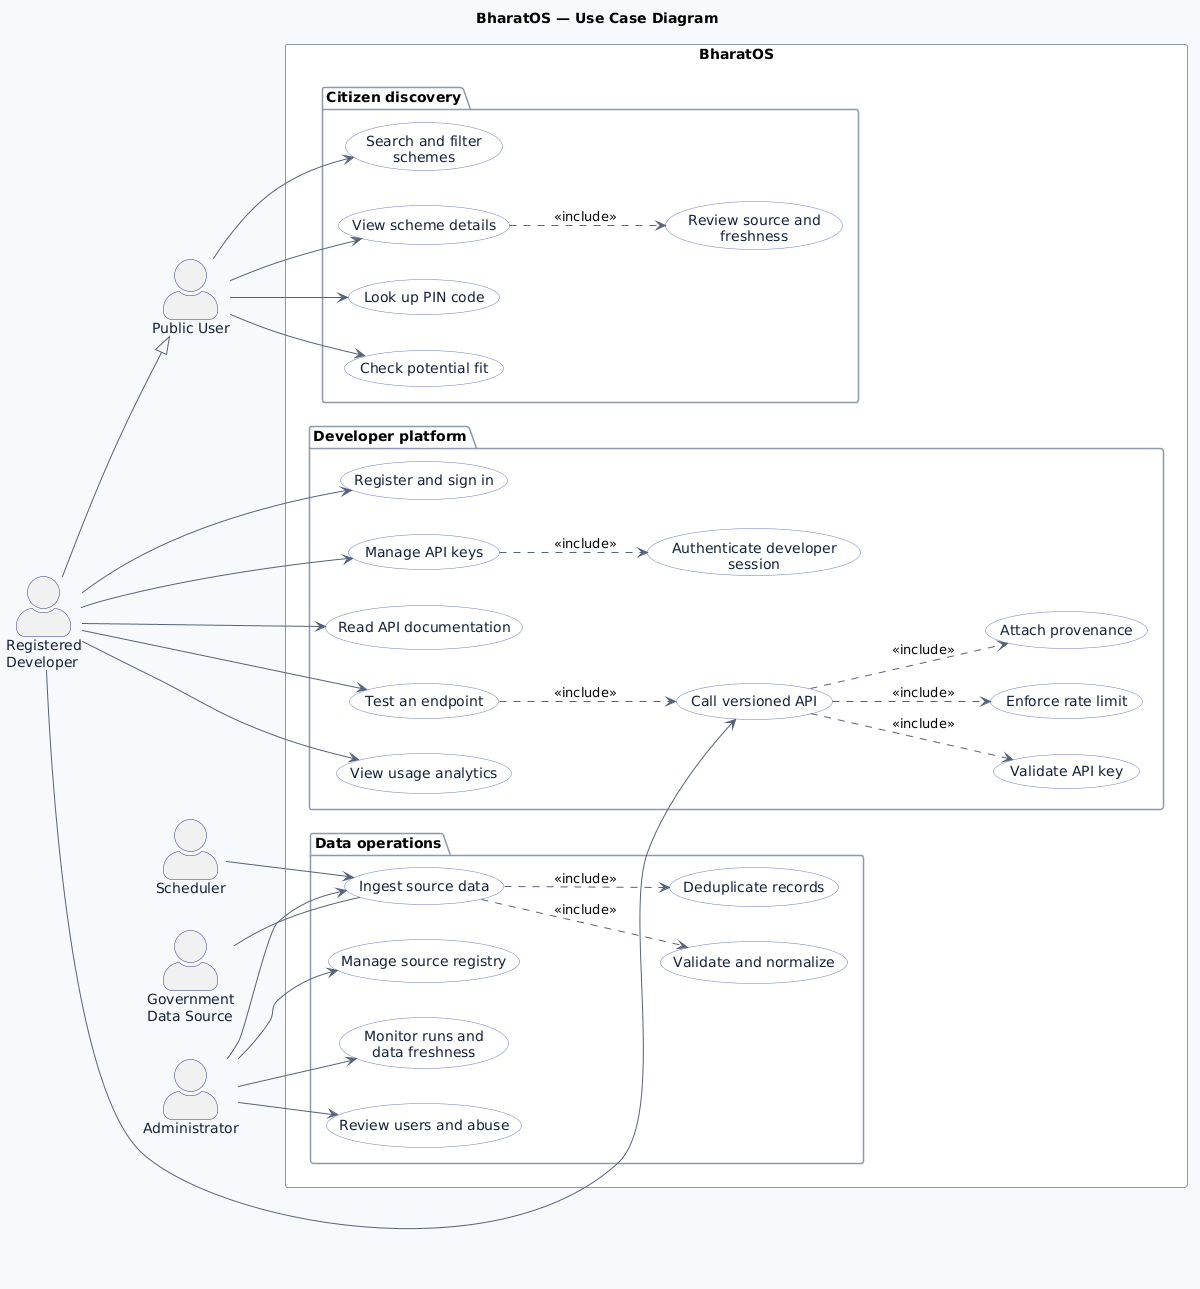
\includegraphics[width=\linewidth,height=0.88\textheight,keepaspectratio]{use-case.png}
\caption{Use Case Diagram for the complete BharatOS target system}
\label{fig:usecase}
\end{figure}
\clearpage

\chapter{Methodology and System Design}

\section{Development Methodology}
The project uses incremental, risk-first development. Phase 1 proves the interface and API
contract with static validated objects. Phase 2 introduces durable normalization and two real
adapters. Later phases add developer identity, cache/rate limits, more datasets, operations and
deployment. Each phase has an observable exit criterion, reducing the risk of building a large
pipeline before its request contract and user experience have been tested.

\section{High-Level Architecture}
The target design separates browser experiences, live request serving and offline ingestion.
The public portal and developer console depend on an API gateway. Authentication, data
services and request logging remain independent services. PostgreSQL is the durable source of
truth; Redis contains disposable response-cache and quota state. The ingestion worker interacts
with external official sources separately from latency-sensitive API serving.

\begin{landscape}
\begin{figure}[p]
\centering
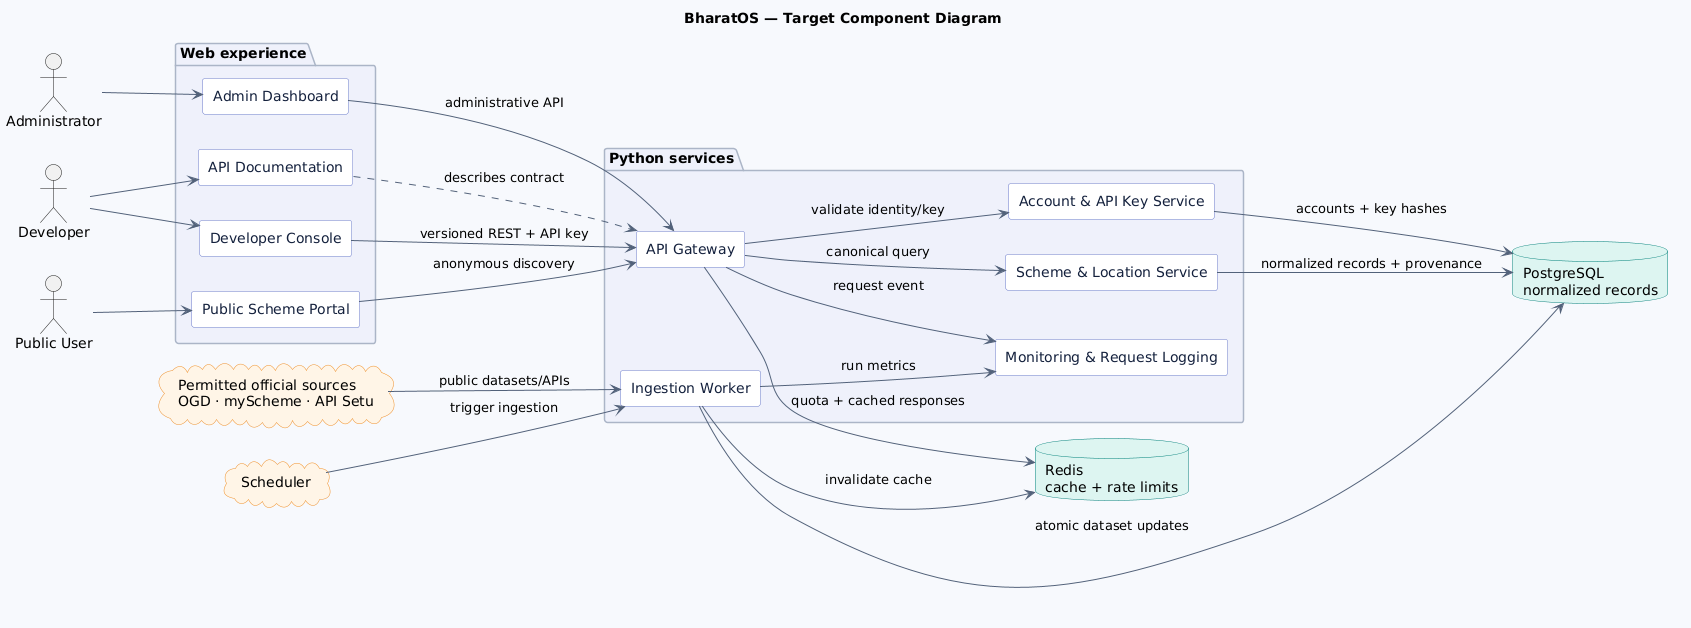
\includegraphics[width=0.95\linewidth,height=0.79\textheight,keepaspectratio]{component.png}
\caption{Component Diagram showing target services and dependencies}
\label{fig:component}
\end{figure}
\end{landscape}

Figure~\ref{fig:component} includes future services so that the design can be defended as a
complete software system. In Phase 1, the Web Application, API Gateway behaviour, Data Service
contract and prototype monitoring surfaces run in one FastAPI process; PostgreSQL, Redis,
schedulers and production authentication are not represented as completed code.

\section{Domain Model and Class Design}
The canonical model is centred on \texttt{NormalizedRecord}. \texttt{Scheme} and
\texttt{Location} inherit shared identifiers and provenance behaviour. \texttt{SourceMetadata}
is composed into normalized records because a record without provenance violates the platform
contract. A scheme composes one or more eligibility rules. Developer accounts aggregate keys,
and each protected request log refers to the key that authorized it.

\clearpage
\begin{figure}[p]
\centering
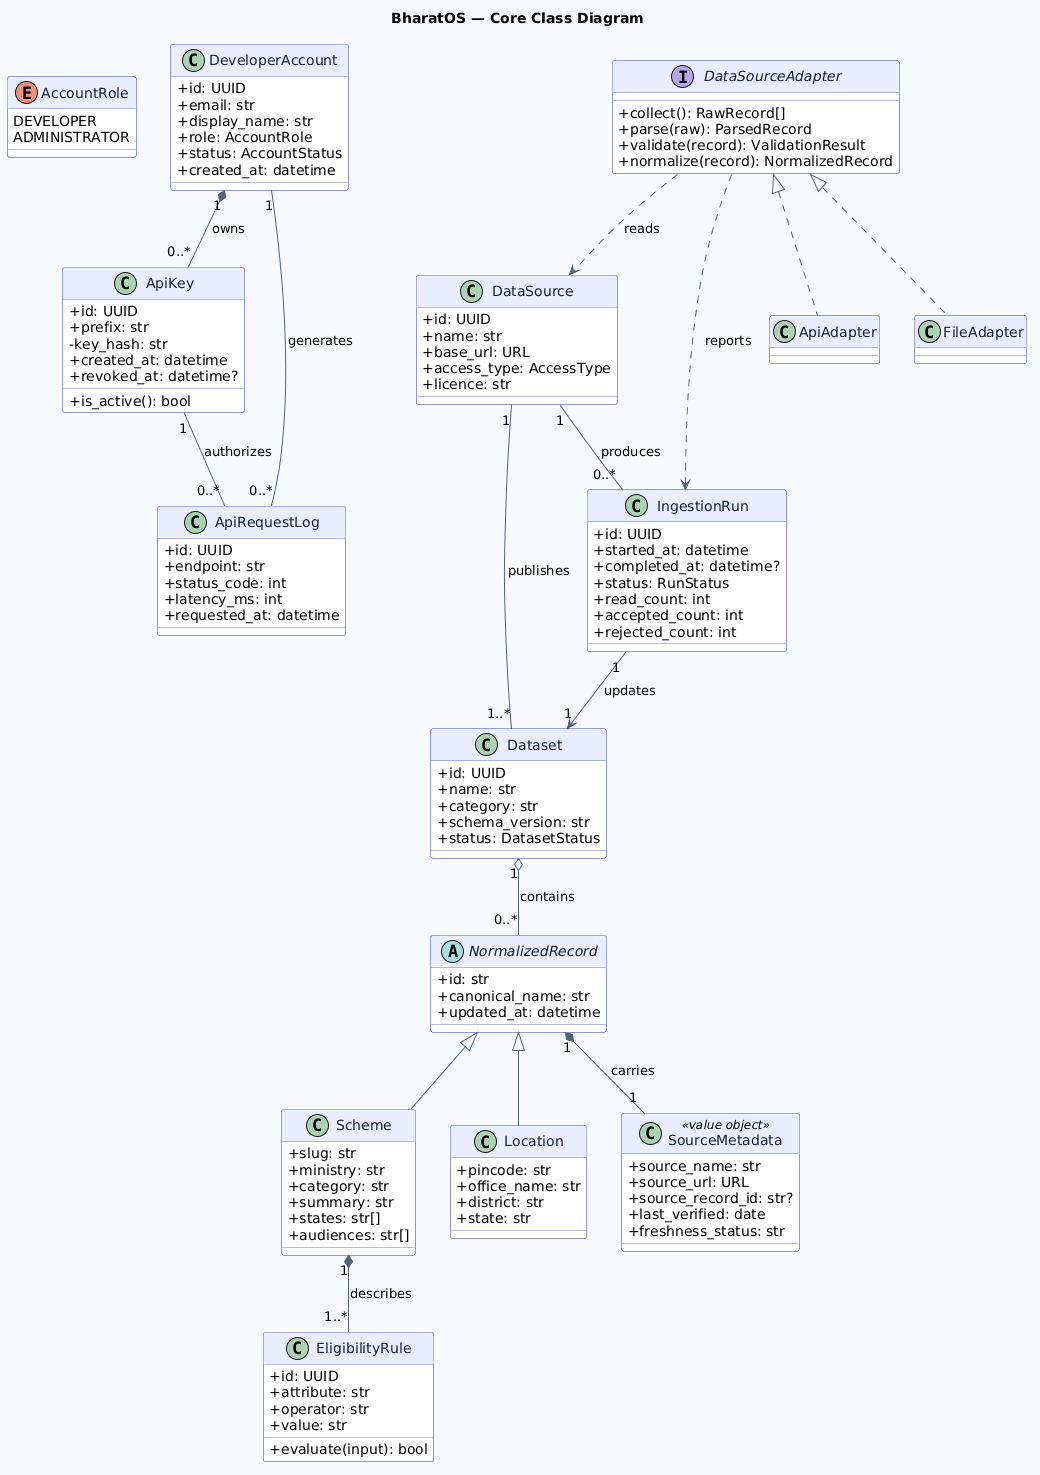
\includegraphics[width=\linewidth,height=0.88\textheight,keepaspectratio]{class.png}
\caption{Class Diagram with inheritance, composition and multiplicities}
\label{fig:class}
\end{figure}
\clearpage

The multiplicities in Figure~\ref{fig:class} are deliberate. One account may own zero or many
keys; a new account can exist before key creation. One key may authorize zero or many requests.
One dataset may initially contain zero records, while a data source publishes one or more
datasets and produces zero or more ingestion runs. The adapter interface isolates API and file
sources behind the same collect, validate and normalize contract.

\section{Protected API Request Sequence}
The gateway validates the presented API key before checking quota. Invalid keys return
\texttt{401}; exhausted quotas return \texttt{429}. Allowed requests check Redis. A cache hit
avoids the data service and database. A cache miss invokes the data service, queries PostgreSQL,
caches the result, writes a request log and returns the standardized envelope.

\clearpage
\begin{figure}[p]
\centering
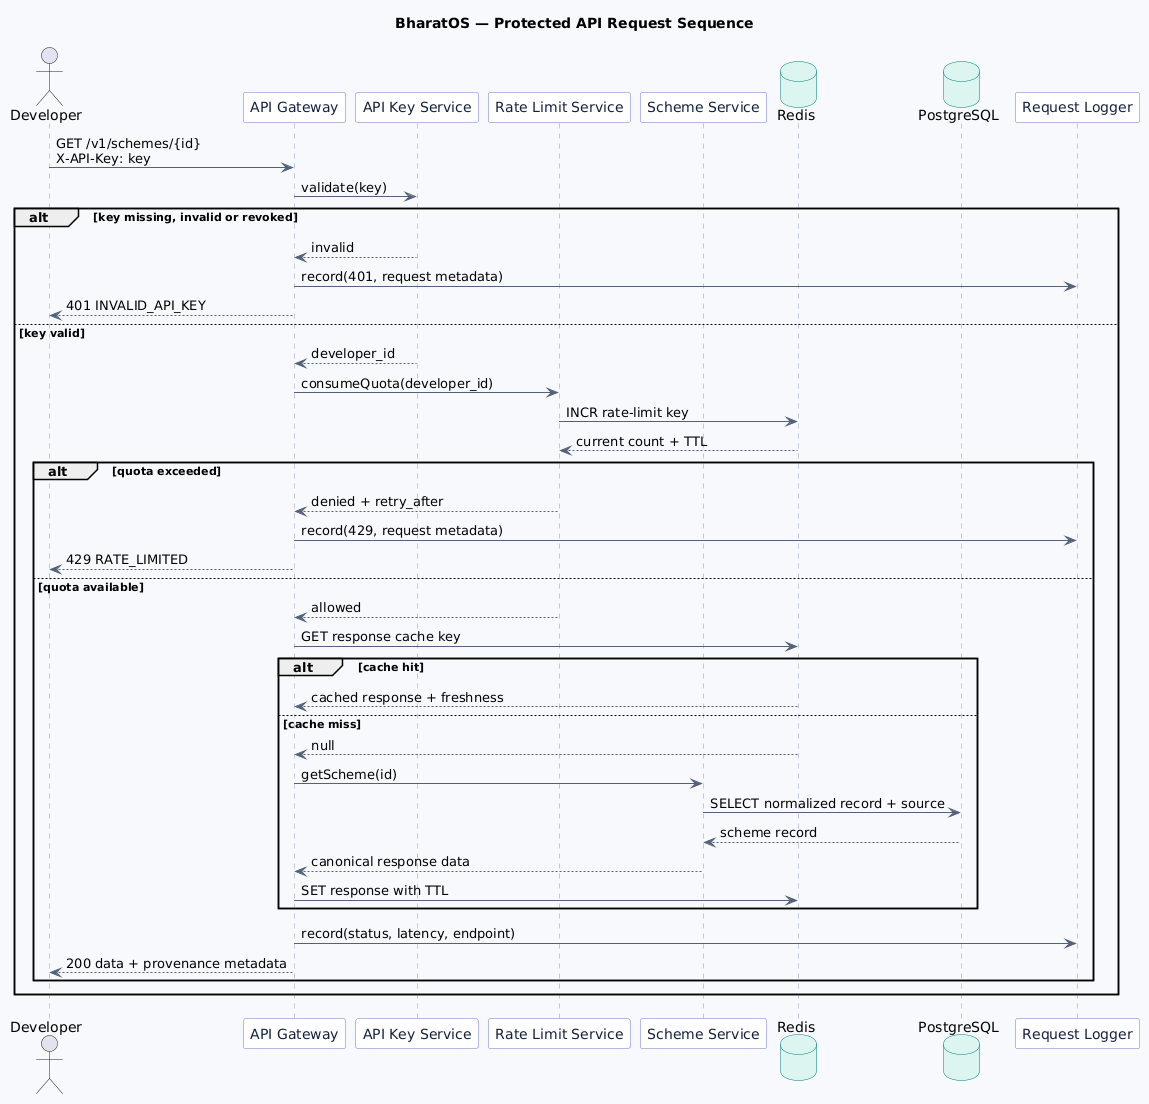
\includegraphics[width=\linewidth,height=0.88\textheight,keepaspectratio]{sequence.png}
\caption{Sequence Diagram for key validation, quota, cache and data access}
\label{fig:sequence}
\end{figure}
\clearpage

The \texttt{alt} fragments in Figure~\ref{fig:sequence} are mutually exclusive decision paths.
Phase 1 implements the key-valid/invalid paths and in-memory data retrieval. Redis, PostgreSQL
and durable request logging are target-phase responsibilities.

\section{Ingestion Activity}
Each source is collected in its native format, parsed and validated. Invalid records are sent to
quarantine with reasons. Valid records are normalized, deduplicated and enriched with source
metadata. A batch is committed only if it satisfies the quality threshold; otherwise it rolls
back for review. A failed source fetch updates source health and marks existing data stale.

\clearpage
\begin{figure}[p]
\centering
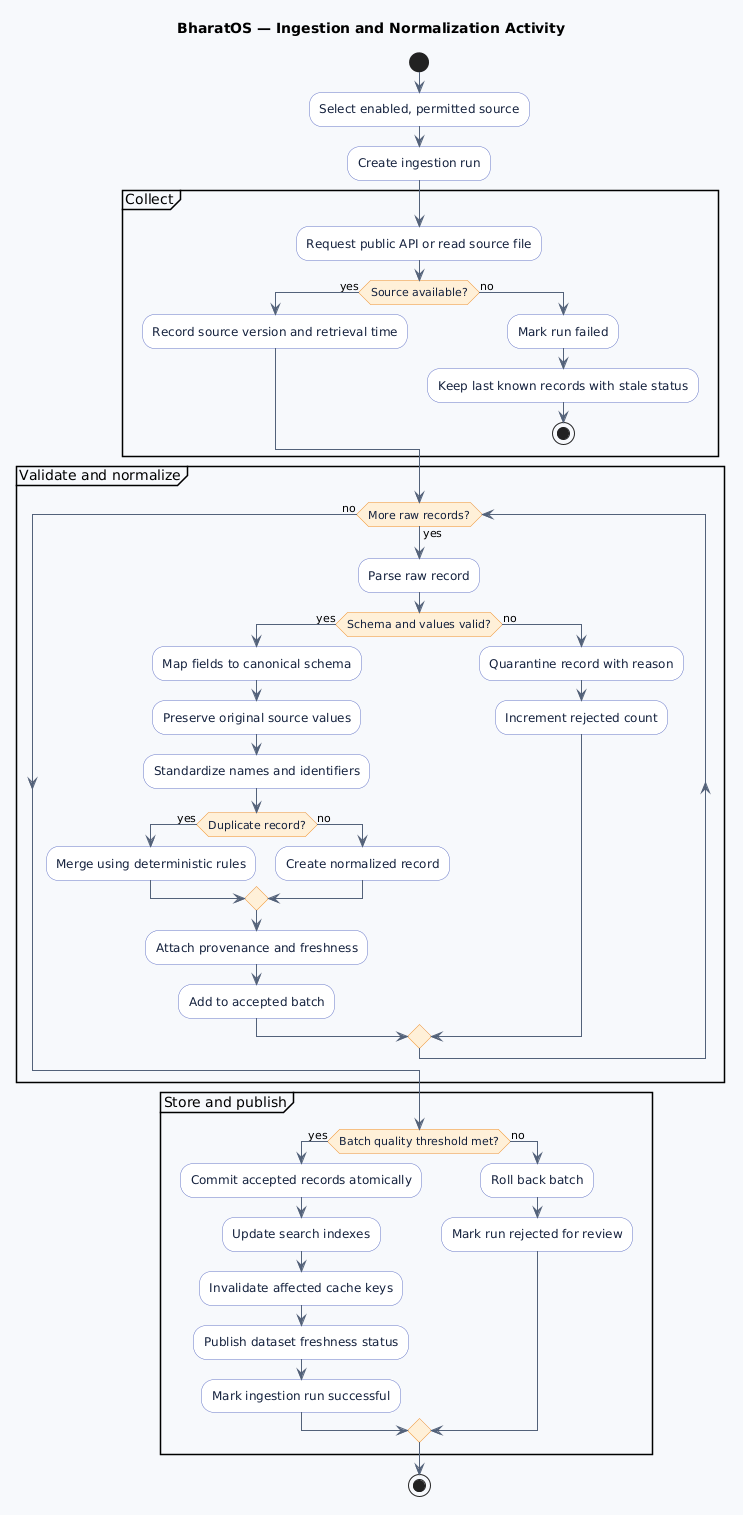
\includegraphics[width=\linewidth,height=0.88\textheight,keepaspectratio]{activity.png}
\caption{Activity Diagram for collect-to-publish ingestion}
\label{fig:activity}
\end{figure}
\clearpage

\section{Technical Stack}
\begin{table}[H]
\centering
\begin{tabularx}{\textwidth}{@{}lXX@{}}
\toprule
\textbf{Layer} & \textbf{Phase 1 technology} & \textbf{Reason} \\
\midrule
Language/runtime & Python 3.12+ & One language for API, validation, ingestion and tests. \\
Web framework & FastAPI & Typed routing, dependency injection and asynchronous capability~\cite{fastapi}. \\
Views & Jinja templates & Server-rendered pages without a Node build pipeline. \\
Validation & Pydantic & Explicit canonical models and deterministic validation~\cite{pydantic}. \\
Browser layer & Custom CSS and minimal JavaScript & Responsive interaction with low complexity. \\
Testing & pytest and FastAPI TestClient & Fast unit and route-level integration checks. \\
Diagramming & PlantUML & Editable, reproducible UML source and SVG/PNG output~\cite{plantuml,uml}. \\
Dependency management & uv & Locked and reproducible Python environment. \\
\bottomrule
\end{tabularx}
\caption{Phase 1 technical stack}
\label{tab:stack}
\end{table}

\section{API Contracts}
Successful responses contain \texttt{data} and \texttt{meta}. The metadata records API version,
prototype environment, source, last verification time, generation time and result count. Errors
contain \texttt{error.code}, \texttt{error.message} and \texttt{error.request\_id}. Versioning
under \texttt{/api/v1} protects current clients from future incompatible schemas.

\noindent\begin{minipage}{\linewidth}
\begin{verbatim}
{
  "data": {},
  "meta": {
    "api_version": "v1",
    "environment": "prototype",
    "source": "Publisher or source set",
    "last_verified": "2026-09-09",
    "generated_at": "ISO-8601 timestamp",
    "result_count": 1
  }
}
\end{verbatim}
\end{minipage}

\chapter{Phase 1 Implementation}

\section{Public Discovery Portal}
The root page displays the academic-prototype disclaimer, free-text search and category, state
and audience filters. Filters are optional and composable. Results show a short scheme summary,
relevant audiences, freshness state and source. Detail pages add ministry, benefits and broad
potential-fit guidance while directing users to the official source for authoritative rules.
No profile, selected filter or personal information is persisted.

\section{Developer Console and API Playground}
The developer page exposes the fixed key \texttt{bharatos\_demo\_2026}, three selectable
endpoints, an optional parameter field and formatted JSON output. Requests are sent to the same
FastAPI routes documented for external clients. A browser-only counter demonstrates the future
usage experience but resets on refresh and is never presented as durable analytics.

\begin{table}[H]
\centering
\begin{tabularx}{\textwidth}{@{}p{2cm}p{6.2cm}X@{}}
\toprule
\textbf{Method} & \textbf{Path} & \textbf{Purpose} \\
\midrule
GET & \texttt{/api/v1/schemes} & Search/filter normalized scheme records. \\
GET & \texttt{/api/v1/schemes/\{scheme\_id\}} & Retrieve one canonical scheme. \\
GET & \path|/api/v1/locations/pincode/{pincode}| & Resolve one six-digit PIN-code record. \\
\bottomrule
\end{tabularx}
\caption{Implemented prototype API endpoints}
\label{tab:endpoints}
\end{table}

\section{Documentation and Administrator Preview}
The documentation page explains authentication, query parameters, response envelopes and the
component diagram. The administrator page clearly labels source status, ingestion stages,
freshness and API statistics as mock values. This distinction lets evaluators inspect the
planned operations surface without mistaking it for connected monitoring.

\section{Prototype Data and Provenance}
Eight scheme records cover agriculture, health, housing, energy, employment, social security
and education. The three PIN-code records provide deterministic developer examples. Each
record contains an official source URL and a verification date of 9 September 2026.

\begin{table}[H]
\centering
\begin{tabularx}{\textwidth}{@{}lXX@{}}
\toprule
\textbf{Records} & \textbf{Source} & \textbf{Prototype use} \\
\midrule
Seven scheme snapshots & myScheme, Digital India Corporation & Names, ministries, broad purpose
and official links. \\
Atal Pension Yojana & Pension Fund Regulatory and Development Authority & Broad purpose, audience
and official source link. \\
Three PIN-code examples & OGD Platform India, Department of Posts & Demonstration location lookup. \\
\bottomrule
\end{tabularx}
\caption{Phase 1 source register}
\label{tab:sources}
\end{table}

\section{Python-first Architecture Decision}
The original proposal suggested Next.js and Node.js. Phase 1 instead uses FastAPI, Jinja and
Pydantic so API serving, data validation, future adapters and automated tests can share one
language. Server rendering avoids a frontend build system, while a small JavaScript module
preserves navigation, copy and playground interactions. The REST contract and layered system
design remain independent of this language choice.

\section{Security, Privacy and Legal Boundaries}
The visible key is suitable only for demonstrating protected-request behaviour on localhost.
Production keys must be random, shown once, stored as hashes, revocable and sent over HTTPS.
Citizen discovery deliberately avoids Aadhaar, PAN, driving-licence verification and saved
profiles. Only permitted public/open sources may be ingested. Stale data must be labelled, and
the interface consistently states that BharatOS is not an official Government of India service
and does not determine eligibility.

\chapter{Results and Evaluation}

\section{Testing Methodology}
\begin{itemize}
  \item \textbf{Model tests:} validate required fields and source metadata using Pydantic.
  \item \textbf{Filter tests:} verify text, category, state and audience combinations.
  \item \textbf{Route tests:} use FastAPI TestClient to check all five pages and three endpoints.
  \item \textbf{Security-contract tests:} verify missing/invalid keys produce standardized
        \texttt{401} envelopes.
  \item \textbf{Boundary tests:} check unknown scheme records and invalid PIN-code formats.
  \item \textbf{Diagram tests:} verify every SVG parses and every PNG has a valid signature.
  \item \textbf{Static checks:} run Ruff over the Python project.
  \item \textbf{Visual checks:} inspect desktop and 390-pixel mobile layouts, navigation,
        filtering and the developer playground.
\end{itemize}

\section{Measured Phase 1 Results}
\begin{table}[H]
\centering
\begin{tabularx}{\textwidth}{@{}X p{3.2cm}p{2.7cm}@{}}
\toprule
\textbf{Acceptance check} & \textbf{Expected} & \textbf{Result} \\
\midrule
Automated test suite & All defined tests pass & 19/19 passed \\
Python static analysis & No Ruff violations & Passed \\
Public/developer/admin/documentation pages & Five usable pages & Passed \\
Mock API surface & Three executable endpoints & Passed \\
UML outputs & Five valid SVG and PNG pairs & Passed \\
Desktop/mobile layout & No clipping or horizontal overflow & Passed \\
Prototype labelling & Visible on every interface & Passed \\
\bottomrule
\end{tabularx}
\caption{Phase 1 acceptance results}
\label{tab:results}
\end{table}

No throughput, p95 latency, cache-hit ratio or production availability claim is made in this
phase. Those measurements require the Phase 2--5 database, cache, logging and performance
harness. Separating verified results from planned metrics protects the validity of the report.

\section{Objective Evaluation}
The interface, typed contract, protected mock endpoints, source attribution, UML set and test
suite satisfy the Phase 1 objectives. The most important outcome is architectural traceability:
each visible feature maps to a route and model today, while diagrams and the phase table identify
where future database, Redis, authentication and ingestion responsibilities belong.

\section{Risks and Mitigations}
\begin{table}[H]
\centering
\begin{tabularx}{\textwidth}{@{}p{4cm}XX@{}}
\toprule
\textbf{Risk} & \textbf{Impact} & \textbf{Mitigation} \\
\midrule
Stale or changed policy data & Misleading discovery & Store verification time, surface freshness
and link to the official source. \\
Unauthorized source use & Legal and trust harm & Ingest only permitted public data
and retain source/licence records. \\
Overstated eligibility & Harmful user decision & Say ``potentially relevant'' and never issue an
official eligibility decision. \\
Credential theft or abuse & API misuse & Hash production keys, use HTTPS, revocation and quotas. \\
Heterogeneous invalid data & Corrupt canonical records & Validate, quarantine, deduplicate and commit
batches atomically. \\
Source outage & Failed refresh & Keep last-known data only with explicit stale status. \\
\bottomrule
\end{tabularx}
\caption{Major risks and planned mitigations}
\label{tab:risks}
\end{table}

\chapter{Phased Roadmap}

\section{Phase 2: Data and Normalization Foundation}
Introduce PostgreSQL, SQLAlchemy, Alembic and repository/service boundaries. Implement the
common DataSourceAdapter and one official scheme adapter plus one location/PIN-code adapter.
The exit criterion is a reproducible ingestion run that serves validated database records.

\section{Phase 3: Developer Access and API Gateway}
Add registration, secure sessions, hashed key generation/rotation/revocation, Redis caching,
per-key rate limiting and persistent request logs. A new developer must be able to create a key,
call the API, see usage and prove revoked/quota-exceeded keys fail correctly.

\section{Phase 4: Dataset Expansion and Discovery Quality}
Add adapters for health, education, employment, agriculture, transport and environment. Add
scheduling, source-specific validation, indexing and data-quality scores while preserving
anonymous discovery and explicit stale-source states.

\section{Phase 5: Operations, Testing and Evaluation}
Connect the administrator view to real ingestion/source-health data. Complete security and
performance suites; measure concurrency at 10, 50, 100 and 500 requests; record p95 latency,
error rate, provenance coverage and developer time-to-first-call.

\section{Phase 6: Deployment and Extensions}
Add Docker Compose, continuous integration, secret management, TLS, backups and operational
documentation. Optional SDK, GraphQL, multilingual and geospatial work begins only after the
REST platform satisfies its measured targets.

\chapter{Conclusion}

\section{Summary of Work}
BharatOS Phase 1 converts the proposal into a demonstrable Python-first software system. It
combines anonymous scheme discovery with a normalized developer API, preserves provenance,
documents future infrastructure and presents clear boundaries between working prototype and
planned production capabilities. Five UML views make the requirements and design explainable
at actor, domain, runtime, process and component levels.

\section{Key Findings}
\begin{itemize}
  \item A server-rendered Python application can provide a polished citizen and developer
        experience without a separate frontend build pipeline.
  \item Provenance and freshness must be part of the canonical response contract, not optional
        page decoration.
  \item Separating ingestion from request serving enables graceful stale-data behaviour when
        an upstream source fails.
  \item Explicit phase boundaries prevent mock dashboards and fixed keys from being mistaken
        for production security or monitoring.
\end{itemize}

\section{Future Work and Recommendations}
The immediate next step is Phase 2: implement PostgreSQL-backed canonical records and two
permitted adapters with deterministic validation and provenance. Real developer identity and
Redis should follow only after database-backed serving is stable. Public deployment must wait
for source-permission review, secure key handling, TLS, backup/recovery and honest stale-data
behaviour.

\section{Final Remarks}
The project demonstrates software engineering through staged delivery, typed contracts,
separation of concerns, testable behaviour and traceable design. Its value is not a claim to
replace official systems, but a disciplined method for making permitted civic information
easier to discover and integrate while keeping the authoritative source visible.

\appendix
\chapter{Demonstration Script}
\begin{enumerate}
  \item State the fragmentation problem and the student-project boundary.
  \item Search for ``health,'' apply an audience filter and open a scheme detail page.
  \item Point out source, freshness and the indicative-eligibility warning.
  \item Open the developer console and run the scheme list, one scheme ID and PIN \texttt{147004}.
  \item Explain the success envelope and the standard \texttt{401} error for a missing key.
  \item Open the administrator preview and distinguish mock values from implemented monitoring.
  \item Use the five diagrams to explain requirements, structure, request flow, ingestion and
        target components.
  \item End with PostgreSQL/ingestion as Phase 2 and secure developer access/Redis as Phase 3.
\end{enumerate}

\chapter{Requirements Traceability}
\begin{table}[H]
\centering
\begin{tabularx}{\textwidth}{@{}p{1.5cm}XX@{}}
\toprule
\textbf{ID} & \textbf{Implementation evidence} & \textbf{Verification} \\
\midrule
FR-01 & Root page and in-memory filter service & Filter and route tests \\
FR-02 & Scheme-detail template and SourceMetadata & Model and route tests \\
FR-03 & Three \texttt{/api/v1} routes & TestClient success-envelope tests \\
FR-04 & API-key dependency and ApiProblem handler & Missing/invalid-key tests \\
FR-05 & Developer console and JavaScript playground & Browser request checks \\
FR-06 & Read-only administrator preview & Page test and visible mock labels \\
FR-07 & Target class/use-case/sequence design & Deferred to Phase 3 \\
FR-08 & Target adapter/activity/component design & Deferred to Phase 2 \\
\bottomrule
\end{tabularx}
\caption{Requirement-to-evidence traceability}
\label{tab:traceability}
\end{table}

\printbibliography[heading=bibintoc]

\end{document}
